\section{Processi primari}
\subsection{Fornitura}
\subsubsection{Obiettivi}
Lo scopo del processo di fornitura è quello di delineare tutte le risorse e le procedure che riguardano l'erogazione del prodotto software che si dovrà realizzare all'interno del progetto. In particolar modo questo processo si pone l'obiettivo di:
\begin{itemize}
	\item stabilire una pianificazione per la fornitura del prodotto finale;
	\item analizzare gli strumenti e le risorse necessarie per candidarsi come fornitori del prodotto;
	\item identificare i bisogni e le necessità del proponente;
	\item definire le caratteristiche e le metriche qualitative del sistema.
\end{itemize}

\subsubsection{Attività}
\paragraph{Avvio}
Il team conduce un analisi preliminare sulla fattibilità del progetto e decide se candidarsi o meno come fornitore del prodotto. Per questa attività è necessario elaborare una corretta analisi costi-benefici per ciascun \textit{capitolato\glo} d'appalto proposto dalle aziende.
\subparagraph*{Studio di fattibilità}
Lo \textit{Studio di Fattibilità 1.1.0\doc} ha lo scopo di analizzare nel dettaglio i capitolati presentati dalle aziende. Il documento,  redatto dagli analisti, è realizzato dopo attenta analisi e discussione da parte dei membri del gruppo nelle apposite riunioni. Per ogni \textit{capitolato\glo} viene indicato:
\begin{itemize}
	\item \textbf{Descrizione Generale}: viene esposto in sintesi il contenuto del \textit{capitolato\glos}, indicando nome del progetto e il proponente;
	\item \textbf{Finalità del Progetto}: viene presentato il \textit{capitolato\glo} dettagliatamente specificando lo scopo del Progetto;
	\item \textbf{Tecnologie Interessate}: vengono elencate le tecnologie coinvolte nel progetto;
	\item \textbf{Aspetti positivi/Criticità}: sono elencati i fattori positivi e di rischio di ciascun \textit{capitolato\glos};
	\item \textbf{Valutazione Conclusiva}: vengono riportate le conclusioni a cui è giunto il team, motivando la scelta o meno del \textit{capitolato\glos}.
\end{itemize}
Il \textit{capitolato\glo} scelto dal gruppo viene evidenziato nella parte introduttiva del documento, nella sezione "Scopo del prodotto".

\paragraph{Proposta e negoziazione del contratto}
A seguito di una richiesta di una prima analisi, il fornitore presenta la proposta formale al cliente. In quanto vincolante, questo contratto dovrà essere opportunamente negoziato o modificato dalle parti in causa.

\paragraph{Pianificazione}  Dovranno essere stabilite le procedure e le risorse necessarie alla realizzazione del prodotto finale. Il fornitore avrà dunque la necessità di elaborare e presentare un \textit{Piano di Progetto 2.2.1\doc} e un \textit{Piano di Qualifica 2.1.1\doc} che ne assicurino la buona riuscita.

\subparagraph*{Piano di Progetto\doc}
Quali attività svolgere e dove allocare le risorse a disposizione è indicato nel \textit{Piano di Progetto}\docs. Il responsabile e gli amministratori di progetto si occuperanno della loro assegnazione, in modo da rendere il \textit{Piano di Progetto 2.2.1\doc} più efficiente possibile. Questo documento deve contenere le seguenti sezioni:
\begin{itemize}
	\item \textbf{Analisi dei rischi}: vengono individuati i possibili rischi e difficoltà che possono palesarsi durante lo svolgimento del progetto. Inoltre, vengono esposti eventuali soluzioni o azioni preventive per evitarli;
	\item \textbf{Modello di sviluppo}: viene definito il metodo di sviluppo scelto e utilizzato per il progetto;
	\item \textbf{Pianificazione}: vengono definite le scadenze temporali per ciascuna attività e i ruoli ai quali assegnare le stesse;
	\item \textbf{Preventivo - Consuntivo}: viene stimato il tempo necessario per ciascuna fase del progetto e, di conseguenza, anche il costo totale del progetto. Viene anche redatto un consuntivo, che riguarda l'andamento effettivo dello stato del progetto e la differenza con ciò che é stato preventivato.
\end{itemize}
\subparagraph*{Piano di Qualifica\doc}
Documento redatto dai verificatori con il compito di delineare le strategie per garantire la qualità del prodotto e dei processi coinvolti durante nel suo ciclo di vita. Il documento sarà così strutturato:
\begin{itemize}
	\item \textbf{Qualità di processo:} sono descritti gli obiettivi e le metriche per garantire la qualità dei processi coinvolti durante il progetto;
	\item \textbf{Qualità di prodotto:} vengono descritte le caratteristiche di qualità principali del sistema. Per ciascuna verranno descritte gli obiettivi e le metriche per misurarle;
	\item \textbf{Test:} sono elencati i tipi di test da eseguire sul sistema. Vengono suddivisi per categoria e sono caratterizzati da un codice univoco, da una descrizione e dal relativo esito;
	\item \textbf{Risultati processo di verifica:} vengono riportati i risultati delle verifiche eseguite mediante l'utilizzo delle apposite metriche e il relativo esito, per ciascuna revisione di avanzamento;
	\item \textbf{Standard e modelli di riferimento:} vengono descritti gli standard e i modelli selezionati per la qualità.
\end{itemize}

\paragraph{Esecuzione e controllo}
Il sistema dovrà essere opportunamente implementato, eseguito e controllato secondo i parametri stabiliti nell'attività di pianificazione.

\paragraph{Revisione e valutazione}
Il fornitore deve verificare e validare il prodotto in modo da assicurare e garantire il soddisfacimento di tutti i requisiti stabiliti per effettuare ciò, il gruppo si impegna ad organizzare degli incontri con l'azienda proponente e con il committente, dimostrando che il prodotto software e i processi attuati soddisfino pienamente i requisiti concordati. Tali incontri saranno possibili tramite le revisioni formali imposte ai fini del progetto didattico e mediante riunioni organizzate con proponente e committente coerentemente con gli incrementi previsti all'interno del \textit{Piano di Progetto}\docs.

\paragraph{Consegna}
Il prodotto deve essere infine consegnato secondo i tempi e le modalità concordate con il committente e il fornitore dovrà garantire assistenza al cliente come previsto dai termini contrattuali. La consegna dovrà essere effettuata rispettando le scadenze e i costi stabiliti nel Piano di Progetto e i vincoli imposti dal Piano di Qualifica.


%\begin{itemize}
%	\item \textbf{Avvio:} il fornitore conduce un analisi preliminare sulla fattibilità del progetto e decide se candidarsi o meno come fornitore del prodotto;
%	\item \textbf{Proposta e negoziazione del contratto:} a seguito di una richiesta di una prima analisi, il fornitore presenta la proposta formale al cliente. In quanto vincolante, questa contratto dovrà essere opportunamente negoziato o modificato dalle parti in causa;
%	\item \textbf{Pianificazione:} dovranno essere stabilite le procedure e le risorse necessarie alla realizzazione del prodotto finale. Il fornitore avrà dunque la necessità di elaborare e presentare un \textit{Piano di Progetto 1.0.0\doc} e un \textit{Piano di Qualifica 1.0.0\doc} che ne assicurino la buona riuscita;
%	\item \textbf{Esecuzione e controllo:} il sistema dovrà essere opportunamente implementato, eseguito e controllato secondo i parametri stabiliti nell'attività di pianificazione;
%	\item \textbf{Revisione e valutazione:} il fornitore dovrà verificare e validare il prodotto insieme al cliente, in modo da assicurare e garantire il soddisfacimento di tutti i requisiti stabiliti;
%	\item \textbf{Consegna:} il prodotto dovrà essere infine consegnato e il fornitore dovrà garantire assistenza al cliente come previsto dai termini contrattuali.
%\end{itemize}

\subsubsection{Procedure}
Per avere ottenere una corretta pianificazione il gruppo ha deciso di agire nel seguente modo:
\begin{enumerate}
	\item identificazione del modello di sviluppo più adatto per il ciclo di vita del prodotto da realizzare (modello incrementale);
	\item individuazione dei processi da adoperare nel ciclo di vita del prodotto e delle attività coinvolte;
	\item analisi dei rischi che si potranno riscontrare nel corso del progetto.
\end{enumerate}
Dopo aver determinato determinato le precedenti caratteristiche, si procederà in maniera ciclica con:
\begin{enumerate}
	\item definizione degli incrementi del modello di sviluppo specificandone obiettivi e task associati;
	\item stima dei costi all'interno del preventivo;
	\item assegnazione dei task per gli incrementi più imminenti ai membri del gruppo;
	\item esecuzione dei task e compimento dell'incremento;
	\item attualizzazione dei rischi (occorrenza e mitigazione);
	\item aggiornamento del consuntivo di periodo;
	\item revisione degli incrementi successivi;
	\item revisione della procedura utilizzata.
\end{enumerate}



\subsubsection{Strumenti}
\paragraph{Microsoft Excel}
Per la creazione degli istogrammi e degli ideogrammi presenti all'interno del \textit{Piano di Progetto 2.2.1\doc} è stato utilizzato il software Microsoft Excel disponibile per tutti i componenti del team mediante la licenza accademica Office 365. Il precedente utilizzo del pacchetto Office da parte dei componenti del gruppo e la sua semplicità hanno favorito la scelta di questo software.
\begin{figure}[h!]
	\caption{Screenshot schermata principale Microsoft Excel}
	\centering
	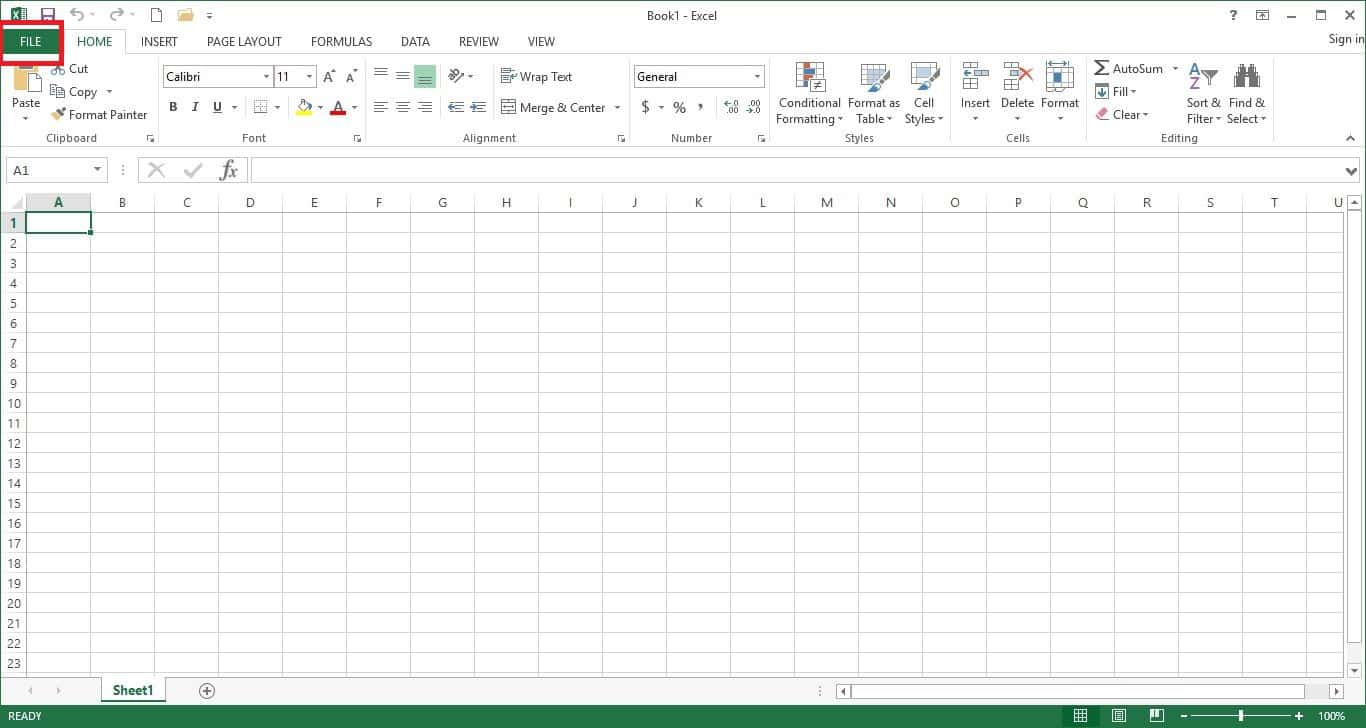
\includegraphics[width=\textwidth]{res/img/excelScreenshot.jpg}
\end{figure}
\newpage
\paragraph{TeamGantt}
Per la creazione dei diagrammi di Gantt è stato utilizzato il software TeamGantt. La scelta di questo software è stata determinata dalle seguenti motivazioni:
\begin{itemize}
	\item semplicità di utilizzo;
	\item possibilità di pianificare le attività con semplici drag and drop;
	\item possibilità di gestire le dipendenze tra i task.
\end{itemize}
\begin{figure}[h!]
	\caption{Screenshot schermata principale TeamGantt}
	\centering
	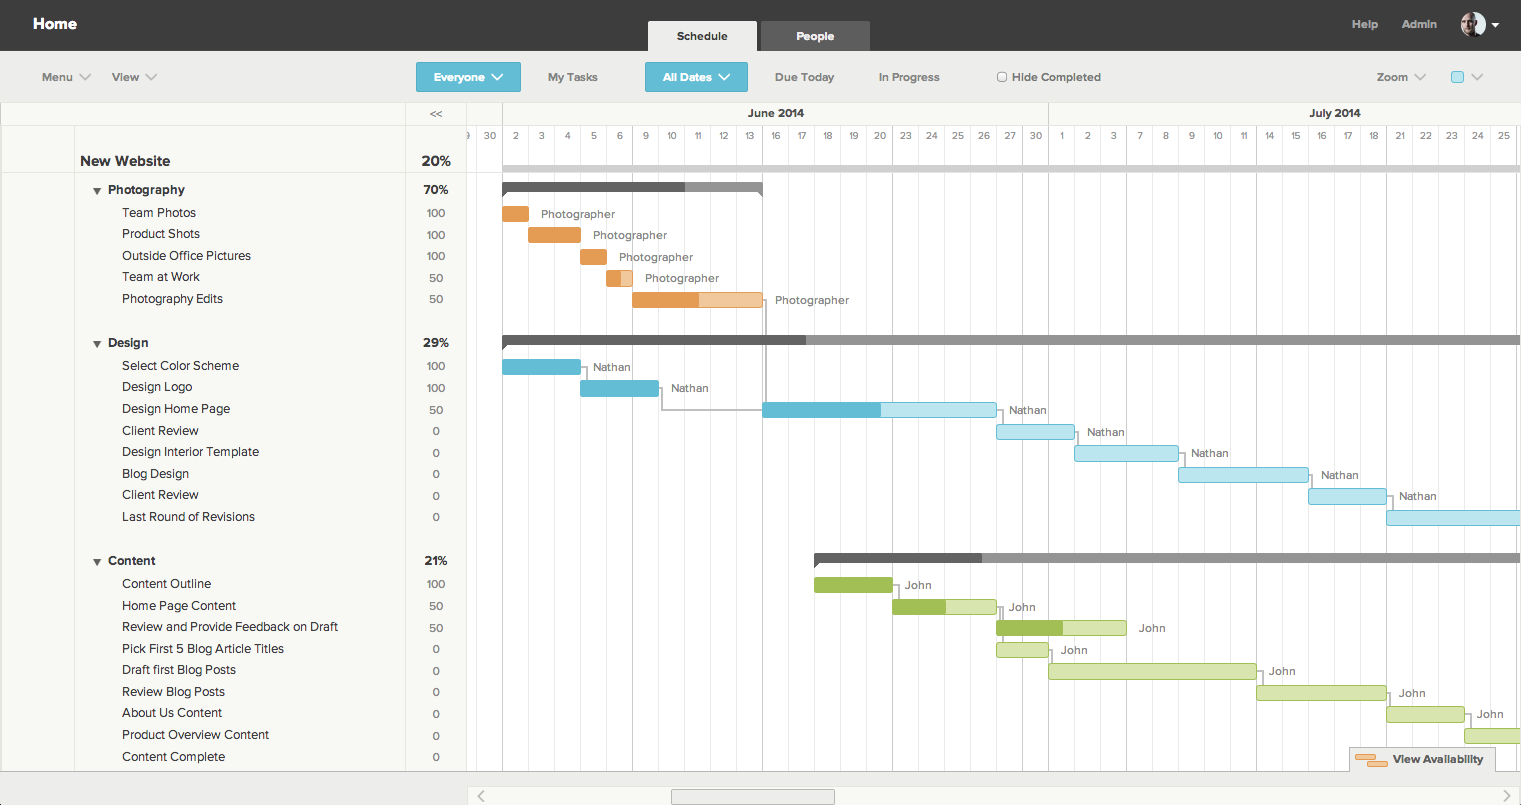
\includegraphics[width=\textwidth]{res/img/teamganttScreenshot.png}
\end{figure}
